Subbab ini menjelaskan perancangan dan implementasi kontroler logika fuzzy Mamdani yang digunakan dalam penelitian ini. \textit{Fuzzy controller} berperan sebagai lapisan adaptif di atas APF \textit{local planner}: alih-alih menggunakan formula \textit{crisp} tetap untuk menentukan kecepatan dan penguatan tolak, \textit{fuzzy controller} menentukan kedua nilai tersebut secara dinamis berdasarkan kondisi lingkungan \textit{real-time}~\cite{Mamdani1974}.

% -----------------------------------------------------------------------
\subsection{Peran Fuzzy dalam Sistem Navigasi}
\label{sec:fuzzy_peran}
% -----------------------------------------------------------------------

Pada konfigurasi \textit{baseline} (S1--S4), APFPlanner menggunakan formula \textit{crisp} bawaan untuk menghitung penguatan gaya tolak:
$G_\text{crisp} = 1{,}0 + (1{,}0 - \tau_\text{trav})$. Formula ini bersifat linear dan tidak memiliki mekanisme untuk memperlambat robot secara proaktif saat lingkungan mulai menyempit atau \textit{obstacle} termal mulai terdeteksi. Akibatnya, robot cenderung bergerak pada kecepatan penuh hingga gaya tolak APF menjadi cukup besar untuk memaksanya berbelok, sehingga menghasilkan jalur yang berpotensi melintas terlalu dekat dengan \textit{obstacle}.

Logika fuzzy mengatasi keterbatasan ini melalui dua mekanisme sekaligus. Pertama, dengan menghasilkan \texttt{rep\_gain} yang bersifat adaptif dan non-linear terhadap kombinasi jarak \textit{obstacle} dan nilai \textit{traversability}. Kedua, dengan menghasilkan \texttt{speed\_scale} yang secara eksplisit mengurangi kecepatan robot lebih awal, sebelum robot terlalu dekat dengan \textit{obstacle}, sehingga tersedia lebih banyak waktu reaksi. Kombinasi keduanya memungkinkan robot mempertahankan margin keamanan (\textit{clearance}) yang lebih besar tanpa harus mengorbankan keberhasilan navigasi~\cite{Haider2022,Benaicha2026}.

Logika fuzzy diimplementasikan sebagai modul \textit{header-only} C++ (\texttt{fuzzy\_controller.h}) yang terintegrasi langsung ke dalam \texttt{APFPlanner}. Modul ini hanya dipanggil pada konfigurasi fuzzy (\texttt{use\_fuzzy = true}, skenario S5--S8). Pada konfigurasi \textit{baseline}, blok pemanggilan fuzzy dilewati sepenuhnya sehingga tidak ada \textit{overhead} komputasi yang membedakan keduanya selain mekanisme kontrol itu sendiri. Desain ini memastikan bahwa seluruh perbedaan performa yang terukur antara konfigurasi \textit{baseline} dan fuzzy benar-benar mencerminkan kontribusi logika fuzzy, bukan artefak implementasi lainnya.

% -----------------------------------------------------------------------
\subsection{Variabel Input dan Output}
\label{sec:fuzzy_var}
% -----------------------------------------------------------------------

Kontroler fuzzy pada penelitian ini menggunakan dua variabel input dan dua variabel output, yang seluruhnya telah diverifikasi dari implementasi \texttt{fuzzy\_controller.h}.

\subsubsection*{a. Input 1 --- Jarak \textit{Obstacle} ($d_\text{obs}$)}

Variabel input pertama adalah jarak minimum ke \textit{obstacle} terdekat yang terdeteksi dari data LiDAR \texttt{/scan}, dalam satuan meter. Nilai ini diklem (\textit{clamp}) secara eksplisit di dalam APFPlanner pada rentang $[0{,}15,\ 2{,}00]$~m. Batas bawah mencegah singularitas matematis pada perhitungan gaya repulsif APF saat $d_\text{obs} \to 0$, sedangkan batas atas membatasi domain sebelum nilai masuk ke inferensi fuzzy. Domain ini dipilih karena APF hanya aktif merespons \textit{obstacle} dalam radius deteksi maksimum \texttt{obs\_detect\_radius} $\leq 1{,}3$~m, dan nilai di atas 2,0~m dianggap sebagai \textit{obstacle} bebas sehingga tidak memerlukan respons.

\subsubsection*{b. Input 2 --- Traversability Efektif ($\tau_\text{eff}$)}

Variabel input kedua adalah nilai $\tau_\text{eff}$ hasil fusi LiDAR--termal yang dijelaskan pada Subbab~\ref{sec:trav_aware}, dibatasi pada rentang $[0{,}00,\ 1{,}00]$. Nilai 0,0 menunjukkan kondisi kritis (koridor sangat sempit atau \textit{obstacle} termal memenuhi area depan), sedangkan nilai 1,0 menunjukkan kondisi aman (koridor lebar dan bebas \textit{obstacle} termal).

\subsubsection*{c. Output 1 --- Skala Kecepatan (\texttt{speed\_scale})}

Variabel output pertama adalah faktor pengali kecepatan linear robot, $\mathit{speed\_scale} \in [0{,}00,\ 1{,}00]$. Nilai 1,0 berarti robot bergerak pada kecepatan penuh ($v_\text{max} = 0{,}2$~m/s), sedangkan nilai 0,0 berarti robot berhenti. Dalam implementasi, $v_x$ dan $v_y$ dikalikan dengan $\mathit{speed\_scale}$ sebelum diterbitkan sebagai \texttt{/cmd\_vel}.

\subsubsection*{d. Output 2 --- Penguatan Repulsi (\texttt{rep\_gain})}

Variabel output kedua adalah faktor penguatan gaya tolak APF, $\mathit{rep\_gain} \in [0{,}50,\ 2{,}50]$. Nilai ini menggantikan $G_\text{crisp}$ pada Persamaan~(\ref{eq:f_rep_scalar}) saat fuzzy aktif. Nilai 0,5 berarti gaya tolak dikurangi (kondisi aman, ruang luas), sedangkan nilai 2,5 berarti gaya tolak diperkuat secara maksimal (kondisi bahaya, ruang sempit atau \textit{obstacle} termal dekat).

\begin{table}[H]
\centering
\caption{Variabel input dan output kontroler fuzzy Mamdani.}
\label{tab:fuzzy_var}
\begin{tabular}{llllp{4.5cm}}
\toprule
\textbf{Jenis} & \textbf{Variabel} & \textbf{Simbol} & \textbf{Domain} & \textbf{Interpretasi} \\
\midrule
Input  & Jarak \textit{obstacle}     & $d_\text{obs}$       & $[0{,}0,\ 2{,}0]$~m & Jarak ke \textit{obstacle} terdekat (LiDAR) \\
Input  & Traversability     & $\tau_\text{eff}$    & $[0{,}0,\ 1{,}0]$   & Kebebasan jalur (fusi LiDAR+termal) \\
Output & Skala kecepatan    & $s_\text{vel}$       & $[0{,}0,\ 1{,}0]$   & Pengali kecepatan linear \\
Output & Penguatan repulsi  & $g_\text{rep}$       & $[0{,}5,\ 2{,}5]$   & Penguatan gaya tolak APF \\
\bottomrule
\end{tabular}
\end{table}

% -----------------------------------------------------------------------
\subsection{Fungsi Keanggotaan}
\label{sec:fuzzy_mf}
% -----------------------------------------------------------------------

Setiap variabel fuzzy didefinisikan menggunakan tiga label linguistik dengan fungsi keanggotaan berbentuk trapesium (\textit{trapmf}) atau segitiga (\textit{trimf}). Bentuk trapesium dipilih untuk label ujung (rendah/lambat/lemah dan tinggi/cepat/kuat) karena memberikan respons jenuh (\textit{saturation}) di area ekstrem, sehingga nilai input yang sangat ekstrem selalu mendapatkan keanggotaan penuh pada label tersebut~\cite{Benaicha2026}. Bentuk segitiga dipilih untuk label tengah karena memberikan transisi yang halus dan simetris.

Fungsi keanggotaan didefinisikan sebagai berikut. Untuk fungsi segitiga:
\begin{equation}
    \mu_\text{trimf}(x;\,a,b,c) =
    \begin{cases}
        0 & x \leq a \\
        \dfrac{x - a}{b - a} & a < x \leq b \\[6pt]
        \dfrac{c - x}{c - b} & b < x \leq c \\
        0 & x > c
    \end{cases}
    \label{eq:trimf}
\end{equation}
dan untuk fungsi trapesium:
\begin{equation}
    \mu_\text{trapmf}(x;\,a,b,c,d) =
    \begin{cases}
        0 & x \leq a \\
        \dfrac{x - a}{b - a} & a < x \leq b \\[4pt]
        1 & b < x \leq c \\[4pt]
        \dfrac{d - x}{d - c} & c < x \leq d \\
        0 & x > d
    \end{cases}
    \label{eq:trapmf}
\end{equation}
Kasus khusus $a = b$ (tepi naik vertikal) atau $c = d$ (tepi turun vertikal) ditangani sebagai nilai langsung 1 atau 0 pada titik tersebut, konsisten dengan implementasi \texttt{skfuzzy.trapmf}.

\subsubsection*{a. Fungsi Keanggotaan Input: Jarak \textit{Obstacle} ($d_\text{obs}$)}

Input jarak didefinisikan dengan tiga label pada domain $[0{,}0,\ 2{,}0]$~m:
\begin{align}
    \mu_\text{dekat}(d)  &= \mu_\text{trapmf}(d;\;0{,}00,\;0{,}00,\;0{,}30,\;0{,}60) \label{eq:mf_dekat} \\
    \mu_\text{sedang}(d) &= \mu_\text{trimf}(d;\;0{,}40,\;0{,}80,\;1{,}20)           \label{eq:mf_sedang_d} \\
    \mu_\text{jauh}(d)   &= \mu_\text{trapmf}(d;\;1{,}00,\;1{,}40,\;2{,}00,\;2{,}00) \label{eq:mf_jauh}
\end{align}
Label \textit{Dekat} memiliki keanggotaan penuh untuk jarak $d \leq 0{,}30$~m dan menurun hingga nol pada $d = 0{,}60$~m. Label \textit{Jauh} mulai naik dari $d = 1{,}00$~m dan mencapai keanggotaan penuh pada $d \geq 1{,}40$~m.

\subsubsection*{b. Fungsi Keanggotaan Input: Traversability ($\tau_\text{eff}$)}

Input traversability didefinisikan dengan tiga label pada domain $[0{,}0,\ 1{,}0]$:
\begin{align}
    \mu_\text{rendah}(\tau) &= \mu_\text{trapmf}(\tau;\;0{,}00,\;0{,}00,\;0{,}25,\;0{,}45) \label{eq:mf_rendah} \\
    \mu_\text{sedang}(\tau) &= \mu_\text{trimf}(\tau;\;0{,}35,\;0{,}55,\;0{,}75)           \label{eq:mf_sedang_t} \\
    \mu_\text{tinggi}(\tau) &= \mu_\text{trapmf}(\tau;\;0{,}60,\;0{,}80,\;1{,}00,\;1{,}00) \label{eq:mf_tinggi}
\end{align}
Label \textit{Rendah} mencakup kondisi ketika jalur banyak terhalang \textit{obstacle} termal atau koridor sempit. Label \textit{Tinggi} mencakup kondisi jalur bebas dan koridor lebar.

\subsubsection*{c. Fungsi Keanggotaan Output: Skala Kecepatan}

Output kecepatan didefinisikan dengan tiga label pada domain $[0{,}0,\ 1{,}0]$:
\begin{align}
    \mu_\text{lambat}(s) &= \mu_\text{trapmf}(s;\;0{,}00,\;0{,}00,\;0{,}15,\;0{,}35) \label{eq:mf_lambat} \\
    \mu_\text{sedang}(s) &= \mu_\text{trimf}(s;\;0{,}30,\;0{,}50,\;0{,}70)           \label{eq:mf_sedang_s} \\
    \mu_\text{cepat}(s)  &= \mu_\text{trapmf}(s;\;0{,}60,\;0{,}80,\;1{,}00,\;1{,}00) \label{eq:mf_cepat}
\end{align}

\subsubsection*{d. Fungsi Keanggotaan Output: Penguatan Repulsi}

Output penguatan repulsi didefinisikan dengan tiga label pada domain $[0{,}5,\ 2{,}5]$:
\begin{align}
    \mu_\text{lemah}(g)  &= \mu_\text{trapmf}(g;\;0{,}5,\;0{,}5,\;0{,}9,\;1{,}3) \label{eq:mf_lemah} \\
    \mu_\text{sedang}(g) &= \mu_\text{trimf}(g;\;1{,}1,\;1{,}5,\;1{,}9)           \label{eq:mf_sedang_g} \\
    \mu_\text{kuat}(g)   &= \mu_\text{trapmf}(g;\;1{,}7,\;2{,}1,\;2{,}5,\;2{,}5) \label{eq:mf_kuat}
\end{align}

Tabel~\ref{tab:fuzzy_mf} merangkum seluruh parameter fungsi keanggotaan dan Gambar~\ref{fig:mf_jarak}--\ref{fig:mf_gain} menampilkan kurva masing-masing variabel.

\begin{table}[H]
\centering
\caption{Parameter fungsi keanggotaan seluruh variabel fuzzy.}
\label{tab:fuzzy_mf}
\begin{tabular}{llllp{4.5cm}}
\toprule
\textbf{Variabel} & \textbf{Label} & \textbf{Tipe} & \textbf{Parameter} & \textbf{Domain} \\
\midrule
\multirow{3}{*}{Jarak ($d$, m)}
  & Dekat  & trapmf & $(0{,}00,\ 0{,}00,\ 0{,}30,\ 0{,}60)$ & $[0{,}0,\ 2{,}0]$~m \\
  & Sedang & trimf  & $(0{,}40,\ 0{,}80,\ 1{,}20)$ & \\
  & Jauh   & trapmf & $(1{,}00,\ 1{,}40,\ 2{,}00,\ 2{,}00)$ & \\
\midrule
\multirow{3}{*}{Traversability ($\tau$)}
  & Rendah & trapmf & $(0{,}00,\ 0{,}00,\ 0{,}25,\ 0{,}45)$ & $[0{,}0,\ 1{,}0]$ \\
  & Sedang & trimf  & $(0{,}35,\ 0{,}55,\ 0{,}75)$ & \\
  & Tinggi & trapmf & $(0{,}60,\ 0{,}80,\ 1{,}00,\ 1{,}00)$ & \\
\midrule
\multirow{3}{*}{Kecepatan ($s$)}
  & Lambat & trapmf & $(0{,}00,\ 0{,}00,\ 0{,}15,\ 0{,}35)$ & $[0{,}0,\ 1{,}0]$ \\
  & Sedang & trimf  & $(0{,}30,\ 0{,}50,\ 0{,}70)$ & \\
  & Cepat  & trapmf & $(0{,}60,\ 0{,}80,\ 1{,}00,\ 1{,}00)$ & \\
\midrule
\multirow{3}{*}{Gain repulsi ($g$)}
  & Lemah  & trapmf & $(0{,}50,\ 0{,}50,\ 0{,}90,\ 1{,}30)$ & $[0{,}5,\ 2{,}5]$ \\
  & Sedang & trimf  & $(1{,}10,\ 1{,}50,\ 1{,}90)$ & \\
  & Kuat   & trapmf & $(1{,}70,\ 2{,}10,\ 2{,}50,\ 2{,}50)$ & \\
\bottomrule
\end{tabular}
\end{table}

\begin{figure}[H]
    \centering
    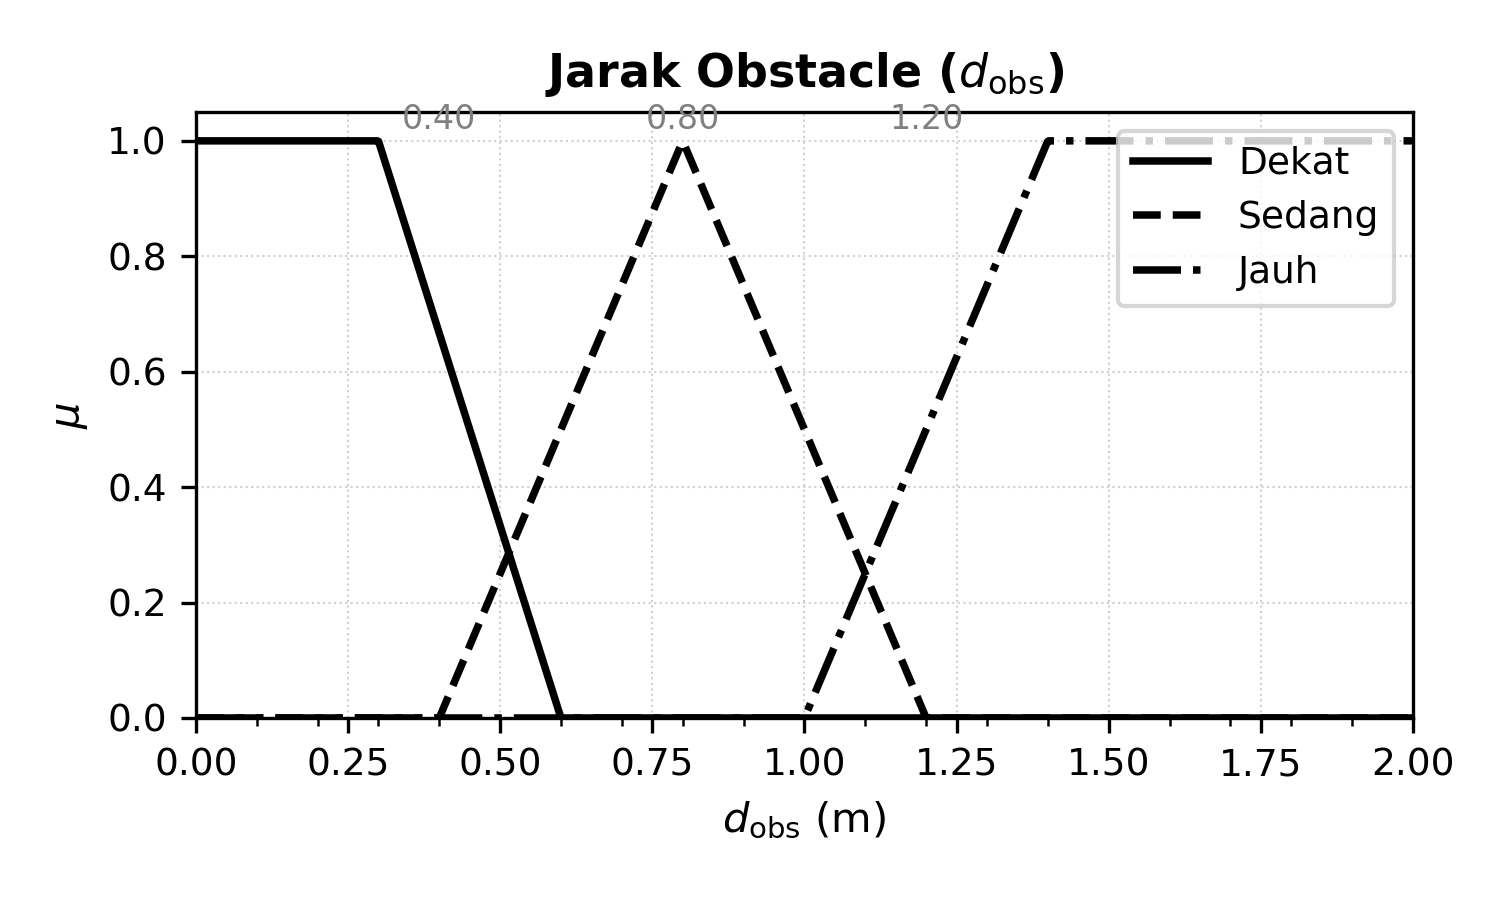
\includegraphics[width=0.48\textwidth]{gambar/3.7_fig_mf_jarak.png} %gambar/fig_mf_jarak
    \hfill
    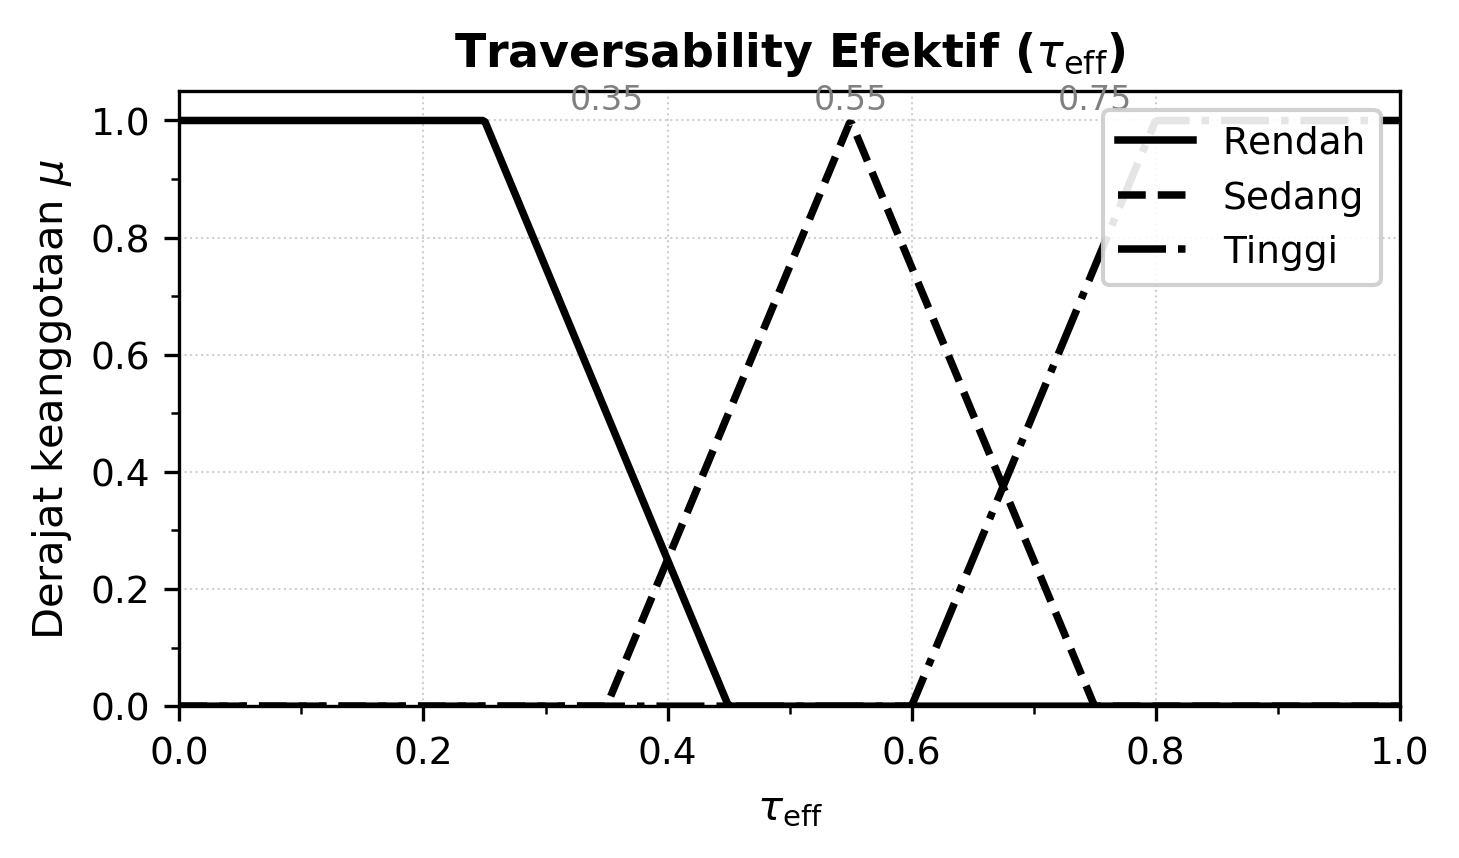
\includegraphics[width=0.48\textwidth]{gambar/3.7_fig_mf_trav.png} %gambar/fig_mf_trav
    \caption{Fungsi keanggotaan variabel input. Kiri: jarak \textit{obstacle} ($d_\text{obs}$, domain $[0, 2]$~m). Kanan: \textit{traversability} efektif ($\tau_\text{eff}$, domain $[0, 1]$).}
    \label{fig:mf_jarak}
\end{figure}

\begin{figure}[H]
    \centering
    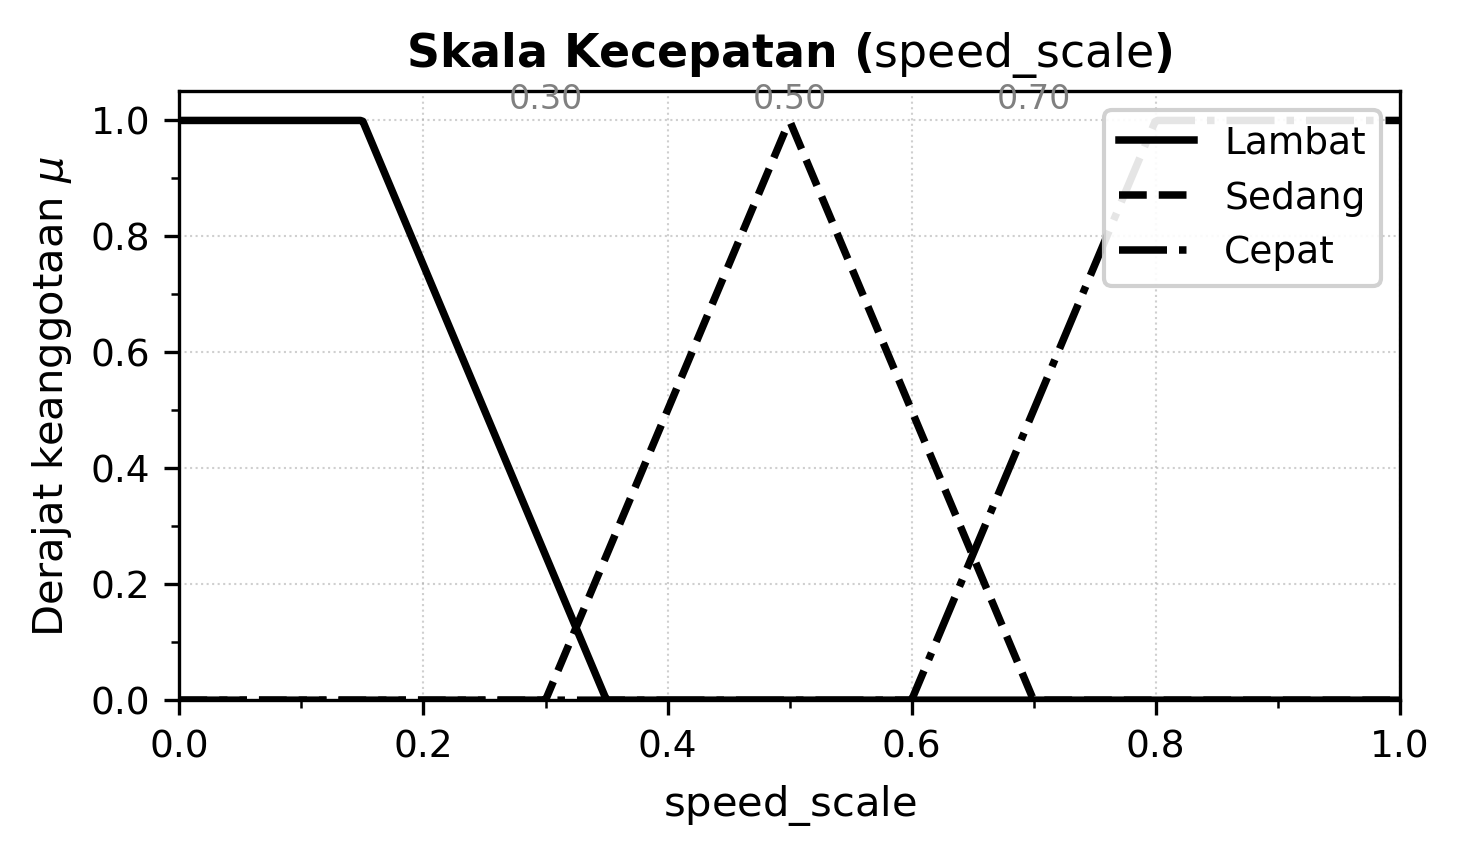
\includegraphics[width=0.48\textwidth]{gambar/3.7_fig_mf_kecepatan.png} %gambar/fig_mf_kecepatan
    \hfill
    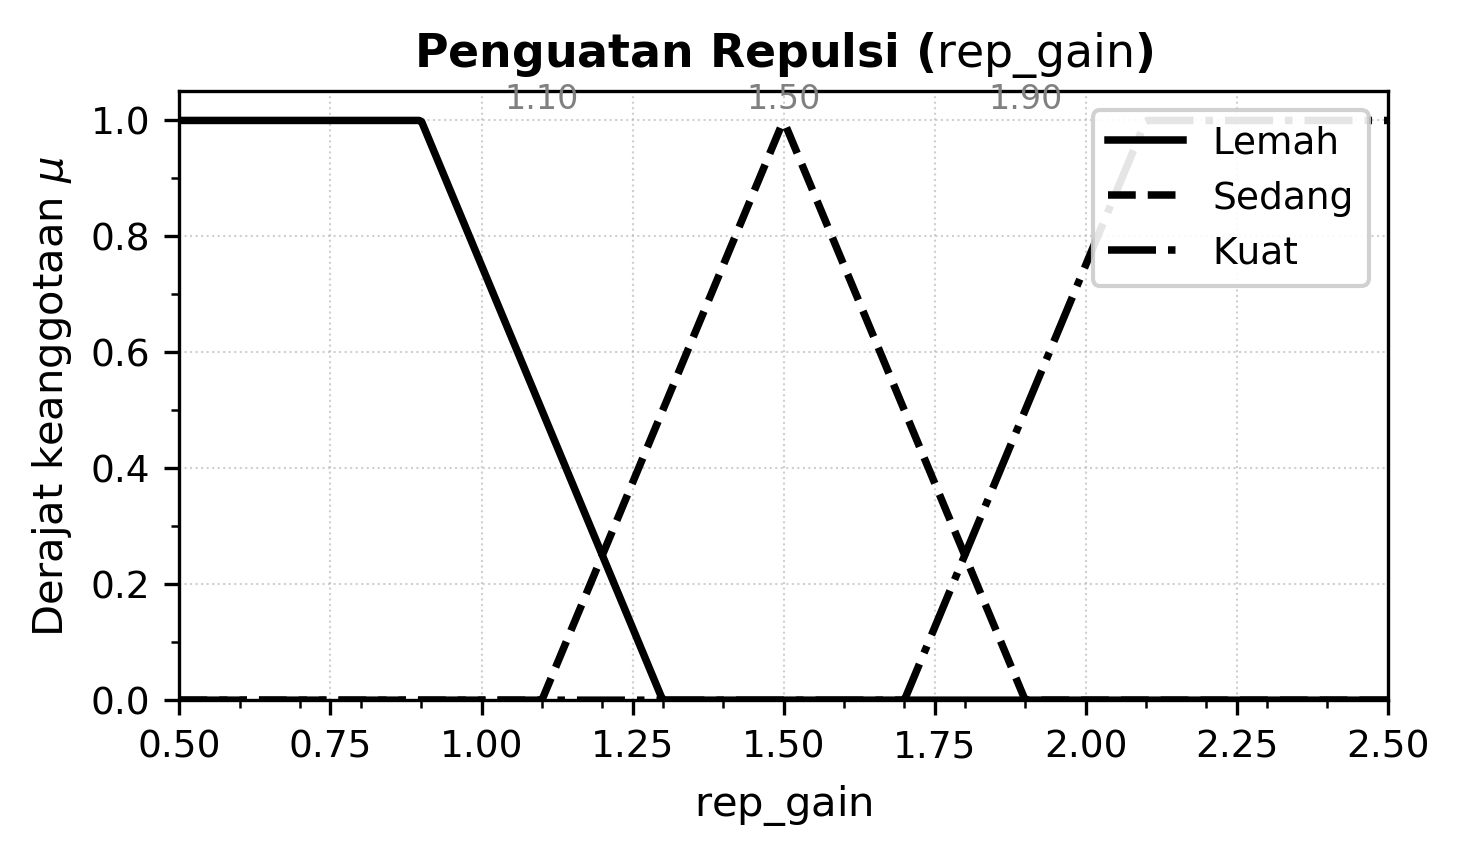
\includegraphics[width=0.48\textwidth]{gambar/3.7_fig_mf_gain.png} %gambar/fig_mf_gain
    \caption{Fungsi keanggotaan variabel output. Kiri: skala kecepatan (\textit{speed\_scale}, domain $[0, 1]$). Kanan: penguatan repulsi (\textit{rep\_gain}, domain $[0{,}5, 2{,}5]$).}
    \label{fig:mf_gain}
\end{figure}

% -----------------------------------------------------------------------
\subsection{Basis Aturan Fuzzy}
\label{sec:fuzzy_rule}
% -----------------------------------------------------------------------

Basis aturan terdiri atas sembilan aturan \textit{IF--THEN} yang mencakup seluruh kombinasi tiga label input pertama (jarak) dengan tiga label input kedua (\textit{traversability}). Desain aturan didasarkan pada dua prinsip navigasi: (1) robot harus melambat dan memperkuat gaya tolak saat \textit{obstacle} dekat atau jalur sempit; (2) robot boleh bergerak cepat dengan gaya tolak lemah saat \textit{obstacle} jauh dan jalur lapang~\cite{Haider2022}.

Tabel~\ref{tab:aturan_fuzzy} menyajikan basis aturan dalam format matriks. Setiap sel berisi pasangan output (\textit{Kecepatan} / \textit{Gain}).

\begin{table}[H]
\centering
\caption{Basis aturan fuzzy Mamdani ($3 \times 3$). Setiap sel: \textit{Kecepatan} / \textit{Gain}. Dikelompokkan berdasarkan kondisi bahaya (merah), transisi (kuning), dan aman (hijau).}
\label{tab:aturan_fuzzy}
\begin{tabular}{lccc}
\toprule
\diagbox{\textbf{Jarak}}{\textbf{Traversability}} &
\textbf{Rendah} & \textbf{Sedang} & \textbf{Tinggi} \\
\midrule
\textbf{Dekat}  & Lambat / Kuat  & Lambat / Kuat  & Sedang / Sedang \\
\textbf{Sedang} & Lambat / Kuat  & Sedang / Sedang & Cepat / Lemah   \\
\textbf{Jauh}   & Sedang / Sedang & Cepat / Lemah  & Cepat / Lemah   \\
\bottomrule
\end{tabular}
\end{table}

Dalam notasi \textit{IF--THEN}, kesembilan aturan tersebut dapat dituliskan sebagai:

\begin{enumerate}
    \item \textbf{IF} jarak \textit{Dekat} \textbf{AND} \textit{traversability} \textit{Rendah}
    \textbf{THEN} kecepatan \textit{Lambat}, gain \textit{Kuat}
    \item \textbf{IF} jarak \textit{Dekat} \textbf{AND} \textit{traversability} \textit{Sedang}
    \textbf{THEN} kecepatan \textit{Lambat}, gain \textit{Kuat}
    \item \textbf{IF} jarak \textit{Dekat} \textbf{AND} \textit{traversability} \textit{Tinggi}
    \textbf{THEN} kecepatan \textit{Sedang}, gain \textit{Sedang}
    \item \textbf{IF} jarak \textit{Sedang} \textbf{AND} \textit{traversability} \textit{Rendah}
    \textbf{THEN} kecepatan \textit{Lambat}, gain \textit{Kuat}
    \item \textbf{IF} jarak \textit{Sedang} \textbf{AND} \textit{traversability} \textit{Sedang}
    \textbf{THEN} kecepatan \textit{Sedang}, gain \textit{Sedang}
    \item \textbf{IF} jarak \textit{Sedang} \textbf{AND} \textit{traversability} \textit{Tinggi}
    \textbf{THEN} kecepatan \textit{Cepat}, gain \textit{Lemah}
    \item \textbf{IF} jarak \textit{Jauh} \textbf{AND} \textit{traversability} \textit{Rendah}
    \textbf{THEN} kecepatan \textit{Sedang}, gain \textit{Sedang}
    \item \textbf{IF} jarak \textit{Jauh} \textbf{AND} \textit{traversability} \textit{Sedang}
    \textbf{THEN} kecepatan \textit{Cepat}, gain \textit{Lemah}
    \item \textbf{IF} jarak \textit{Jauh} \textbf{AND} \textit{traversability} \textit{Tinggi}
    \textbf{THEN} kecepatan \textit{Cepat}, gain \textit{Lemah}
\end{enumerate}

Perlu dicatat bahwa aturan 1 dan 2 (\textit{Dekat--Rendah} dan \textit{Dekat--Sedang}) menghasilkan keluaran yang identik (\textit{Lambat/Kuat}). Hal ini disengaja: ketika robot sangat dekat dengan \textit{obstacle}, seberapa lapang pun jalur secara termal, prioritas utama adalah mengurangi kecepatan dan memperbesar gaya tolak untuk memastikan keselamatan. Sebaliknya, aturan 8 dan 9 (\textit{Jauh--Sedang} dan \textit{Jauh--Tinggi}) juga identik: ketika \textit{obstacle} jauh, kondisi \textit{traversability} sudah tidak terlalu memengaruhi perilaku, sehingga robot diizinkan bergerak cepat dengan gaya tolak minimal.

% -----------------------------------------------------------------------
\subsection{Inferensi dan Defuzzifikasi}
\label{sec:fuzzy_infer}
% -----------------------------------------------------------------------

Proses inferensi fuzzy Mamdani pada penelitian ini mengikuti empat tahap standar, yaitu fuzzifikasi, evaluasi aturan, agregasi, dan defuzzifikasi. Seluruh tahap diimplementasikan secara identik dengan \texttt{scikit-fuzzy} versi 0.5.0, yang telah diverifikasi dengan kesalahan maksimum $|\Delta| < 5 \times 10^{-6}$ pada 588 titik uji~\cite{Mamdani1974}.

\subsubsection*{a. Fuzzifikasi}

Pada setiap siklus kontrol, nilai \textit{crisp} input $d_\text{obs}$ dan $\tau_\text{eff}$ diubah menjadi derajat keanggotaan terhadap masing-masing label. Untuk input jarak, misalnya:
\begin{equation}
    \mu_\text{dekat}(d),\quad \mu_\text{sedang}(d),\quad \mu_\text{jauh}(d)
    \label{eq:fuzz_input}
\end{equation}
menggunakan Persamaan~(\ref{eq:mf_dekat})--(\ref{eq:mf_jauh}) yang telah didefinisikan.

\subsubsection*{b. Evaluasi Aturan --- Operator AND Minimum}

Kekuatan setiap aturan $w_k$ diperoleh menggunakan operator AND berupa nilai minimum antara derajat keanggotaan kedua anteseden:
\begin{equation}
    w_k = \min\!\bigl(\mu_{A_k}(d_\text{obs}),\; \mu_{B_k}(\tau_\text{eff})\bigr),
    \quad k = 1, 2, \ldots, 9
    \label{eq:rule_strength}
\end{equation}
dengan $\mu_{A_k}$ dan $\mu_{B_k}$ adalah fungsi keanggotaan anteseden pertama (jarak) dan kedua (\textit{traversability}) untuk aturan ke-$k$.

\subsubsection*{c. Implikasi Mamdani --- \textit{Clipping}}

Pada metode Mamdani, konsekuen setiap aturan berupa \textit{clipped membership function}: MF output dipotong pada level $w_k$~\cite{Mamdani1974}. Untuk setiap label output $j$ (misalnya \textit{Lambat, Sedang, Cepat} untuk kecepatan), nilai yang di-\textit{clip} pada titik $s$ adalah:
\begin{equation}
    \tilde{\mu}_j(s) = \min \!\bigl(w_k,\; \mu_j(s)\bigr)
    \label{eq:mamdani_clip}
\end{equation}

\subsubsection*{d. Agregasi --- Operator Maksimum}

Kontribusi seluruh aturan yang menghasilkan konsekuen yang sama diagregasikan menggunakan operator maksimum. Aktivasi gabungan untuk setiap label output adalah:
\begin{equation}
    A_j = \max_{k:\,\text{aturan } k \to j}\!\bigl(w_k\bigr)
    \label{eq:aggregation}
\end{equation}
Berdasarkan tabel aturan (Tabel~\ref{tab:aturan_fuzzy}):
\begin{align}
    A_\text{Lambat} &= \max(w_1, w_2, w_4) \label{eq:agg_lambat} \\
    A_\text{Sedang} &= \max(w_3, w_5, w_7) \label{eq:agg_sedang} \\
    A_\text{Cepat}  &= \max(w_6, w_8, w_9) \label{eq:agg_cepat}
\end{align}
dan identik untuk output gain (\textit{Kuat, Sedang, Lemah}).

\subsubsection*{e. Defuzzifikasi --- \textit{Centroid of Gravity}}

Nilai \textit{crisp} output diperoleh menggunakan metode \textit{Centroid of Gravity} (CoG), yang menghitung titik tengah massa dari fungsi keanggotaan yang sudah diagregasikan:
\begin{equation}
    y^* = \frac{\displaystyle\int_{y_\text{min}}^{y_\text{max}}
          y\cdot\mu_\text{agg}(y)\;\mathrm{d}y}
         {\displaystyle\int_{y_\text{min}}^{y_\text{max}}
          \mu_\text{agg}(y)\;\mathrm{d}y}
    \label{eq:defuzz_cog}
\end{equation}
dengan $\mu_\text{agg}(y) = \max\!\bigl(\tilde{\mu}_\text{Lambat}(y),\,
\tilde{\mu}_\text{Sedang}(y),\, \tilde{\mu}_\text{Cepat}(y)\bigr)$ sebagai fungsi keanggotaan agregat pada titik $y$ dalam domain output.

Dalam implementasi C++, integral dievaluasi menggunakan metode piecewise-linear eksak pada grid dengan resolusi 0,01 yang diinterpolasi pada titik-titik potong MF untuk akurasi maksimum, meniru persis algoritma \texttt{skfuzzy.defuzz('centroid')}. Tabel~\ref{tab:fuzzy_verify} menyajikan empat titik verifikasi yang mengonfirmasi kesesuaian implementasi C++ dengan \textit{scikit-fuzzy}.

\begin{table}[H]
\centering
\caption{Verifikasi output \textit{fuzzy controller} pada empat titik uji. Nilai dihasilkan oleh implementasi C++ (\texttt{fuzzy\_controller.h}) dan identik dengan \textit{scikit-fuzzy} 0.5.0 ($|\Delta| < 5 \times 10^{-6}$).}
\label{tab:fuzzy_verify}
\begin{tabular}{ccccc}
\toprule
\textbf{$d_\text{obs}$ (m)} & \textbf{$\tau_\text{eff}$} &
\textbf{\textit{speed\_scale}} & \textbf{\textit{rep\_gain}} &
\textbf{Interpretasi} \\
\midrule
0,50 & 0,25 & 0,159 & 2,131 & Dekat, jalur sempit $\rightarrow$ lambat, gain kuat \\
1,60 & 0,90 & 0,844 & 0,811 & Jauh, jalur bebas $\rightarrow$ cepat, gain lemah  \\
0,80 & 0,55 & 0,500 & 1,500 & Sedang, jalur sedang $\rightarrow$ keduanya sedang \\
0,40 & 0,85 & 0,500 & 1,500 & Dekat namun jalur bebas $\rightarrow$ sedang        \\
\bottomrule
\end{tabular}
\end{table}

Baris ketiga dan keempat pada Tabel~\ref{tab:fuzzy_verify} menunjukkan fenomena menarik: meskipun kondisi input berbeda (jarak 0,80 m dengan \textit{traversability} sedang versus jarak 0,40 m dengan \textit{traversability} tinggi), keduanya menghasilkan output yang identik (\textit{speed\_scale} = 0,500 dan \textit{rep\_gain} = 1,500). Hal ini merupakan konsekuensi alami dari desain aturan yang simetris dan merupakan perilaku yang diinginkan: pada kondisi jarak sangat dekat namun jalur bebas, sistem memberikan respons moderat, yakni lebih hati-hati daripada bergerak cepat, namun tidak menghentikan robot sepenuhnya.